\documentclass[11pt,a4paper]{article}
\usepackage[margin=2.2cm]{geometry}
\usepackage[T1]{fontenc}
\usepackage[utf8]{inputenc}
\usepackage{lmodern}
\usepackage{booktabs}
\usepackage{tabularx}
\usepackage{graphicx}
\usepackage{xcolor}
\usepackage{tikz}
\usetikzlibrary{arrows.meta,positioning}
\usepackage[numbers,sort&compress]{natbib}
\usepackage[colorlinks=true,linkcolor=blue!50!black,citecolor=blue!50!black,urlcolor=blue!50!black]{hyperref}

% Values still to be filled from ml/results/report.md are marked in red.
\newcommand{\todo}[1]{\textcolor{red}{[#1]}}

\title{Automated Quality Assessment of Customer-Support Dialogues\\with a Small Local Language Model}
\author{Aslan Zhumazhanov \and Temirlan Zholtayev \and Alikhan Khamidulla\\[2pt]
\small AI Essentials: Theory and Applications --- final project}
\date{November 2026}

\begin{document}
\maketitle

\begin{abstract}
Contact centres check operator quality with a checklist, but reviewers read only a small sample of
dialogues. We build a system that grades every chat and call (Russian, Kazakh, English) against an
eight-criterion checklist with an open-weight 9B model on a laptop GPU, so that no dialogue leaves the
machine. Instead of asking the model for a verdict, the pipeline splits each criterion into narrow yes/no
questions with a cited message, confirms damaging answers on the cited message, and derives verdicts and
scores with deterministic rules. On 13 held-out dialogues labelled by an annotator outside development
(104 labels) the pipeline agrees with the human on 85.6\% of labels (95\% CI 76.9--93.3\%), against
69.2\% for the standard one-prompt LLM-as-a-judge baseline with the same model (paired difference
$+16.3$ points, CI $+5.8$ to $+26.9$), at 35\,s per dialogue and zero cost. We report confidence intervals, an error analysis, a resource study and the limitations, the most
important being the small test set.
\end{abstract}

\section{Problem and success criteria}
\paragraph{Users and task.} A quality reviewer in a broker's contact centre fills a checklist for a dialogue:
(01) establishing contact, (02) needs discovery, (03) identification, (04) correct and complete consultation,
(05) empathy, (06) dialogue management, (07) closing, (08) gross violations. Criteria 01, 05, 08 are yes/no;
02, 03, 07 are yes/no/N/A; 04 is a scale \{0,5,10,15,20\} or N/A; 06 a scale \{0,4,7,10\}. The final score is
$100\cdot\sum_i w_i s_i/\sum_i w_i$ over applicable criteria (weights 10, 15, 20, 20, 15, 15, 5); 08 is
reported as a flag. Reviewers cover only a sample; the goal is to grade every dialogue and route only the
disputed ones to a person.

\paragraph{Why an LLM, and the constraints.} The criteria are natural-language rules applied to free text in
three languages, and there is no labelled corpus large enough to train a classifier per criterion. A
pretrained instruction-following model can apply written rules without training data. The constraints are:
dialogues contain personal and financial data (they should not leave the company), the hardware is a
laptop GPU with 8\,GB, and every verdict must be checkable by a person.

\paragraph{Success criteria} (fixed before the final test): (i) agreement with a human reviewer
$\geq 85\%$ of checklist labels on unseen dialogues; (ii) every non-N/A verdict cites a message of the
dialogue; (iii) $\leq 60$\,s per dialogue on the 8\,GB GPU; (iv) zero cost and no data sent outside.

\section{Related work}
Using a strong LLM as an evaluator (\emph{LLM-as-a-judge}) was popularised by MT-Bench and Chatbot
Arena~\cite{zheng2023judging}, which also documented position, verbosity and self-enhancement biases;
judges are sensitive to answer order~\cite{wang2024fair}. G-Eval~\cite{liu2023geval} improves agreement with
humans by asking for chain-of-thought~\cite{wei2022cot} before a form-filling score. Prometheus~\cite{kim2024prometheus}
fine-tunes an open model to grade against a user-given rubric. Closest to our design are approaches that
decompose evaluation into small verifiable units: CheckEval~\cite{lee2024checkeval} replaces a holistic score
by a checklist of boolean questions, and FActScore~\cite{min2023factscore} scores atomic facts separately.
We apply the same idea to a domain checklist, but let deterministic rules---not the model---combine the
answers, and require every answer to point to a message, enforced by constrained decoding~\cite{willard2023guided}.
Our baseline is the standard one-prompt judge of~\cite{zheng2023judging,liu2023geval} with reasoning before
each answer.

\section{Data}
\begin{table}[h]\centering\small
\begin{tabularx}{\linewidth}{lXXl}
\toprule
Set & Content & Labels & Use\\
\midrule
DEV & 65 dialogues: 60 chats (RU 30, KZ 15, EN 15), 5 transcribed RU calls & 19 dialogues by the team & development\\
DEV-LLM & 15 other DEV chats + 5 calls & Gemini Pro, spot-checked by an AI assistant, not by a person & development only\\
TEST & 13 dialogues (RU 6, KZ 4, EN 3; 11 chats, 2 calls) & external annotator, written before the model ran & final evaluation\\
TEST-NEW & same 13 dialogues & 4 criteria never seen in development & generalisation\\
\bottomrule
\end{tabularx}
\caption{Data sets. DEV and the checklist were provided by the case owner; TEST was written and labelled by
an annotator who did not take part in developing the pipeline.}
\end{table}

Each record has a conversation id, channel, language and a transcript of messages with a speaker role
(client, operator, bot, system) and a timestamp. Bot messages and system events (``identity verified'',
``operator closed the chat'') are context, not graded. Preprocessing: attachments and tags are dropped,
messages are numbered and rendered as \texttt{M$k$ [role, time]: text}; facts that need no model (first operator
message, language of each message by script and Kazakh-specific letters, pauses, system events) are
extracted by code.

\paragraph{Analysis} (\texttt{ml/eval/data\_analysis.py}, full output in \texttt{ml/results/data\_analysis.md}).
DEV dialogues have 11--115 messages (median 14) and 769--5\,089 characters; TEST 11--26 messages (median 16).
Only 27\% (DEV) and 23\% (TEST) of the messages are written by the operator, who is the one being graded;
the rest are client, bot and system messages. Labels are imbalanced: in TEST, 08 (gross violation) is
``yes'' in 1 of 13 dialogues, 03 is N/A in 9 of 13, and 15\% of all labels are N/A. Exact-match agreement on a
rare class is therefore not informative on its own, and we report the gross-violation flag separately. The
personal-data rules did not fire on any of the 1\,268 DEV messages (Section~\ref{sec:responsible}).

\paragraph{Duplicate and leakage check.} We compared every TEST dialogue with every DEV dialogue by the
Jaccard similarity of word 3-gram sets. On whole transcripts one TEST dialogue looked suspicious (0.556,
above the largest similarity between two DEV dialogues, 0.504), but the similarity came from bot and
system templates shared by all dialogues. On client and operator messages only, the nearest DEV dialogue
scores at most 0.042 for any TEST dialogue, within the range seen between two different DEV dialogues
(nearest-neighbour similarity: median 0.030, 90th percentile 0.061, maximum 0.076), and no client or
operator message longer than 40 characters appears in both sets. We conclude that TEST is not a copy or edit of DEV dialogues.

\paragraph{Leakage control.} Prompts, rules and thresholds were developed on DEV only. TEST was used for
scoring after development, with one documented exception: after the first TEST run the rule for criterion
02 was changed (overall agreement 81.7\%\,$\rightarrow$\,85.6\%). The comparison in Section~\ref{sec:results}
uses the same final code for both systems, so the change does not favour either of them, but the absolute
number is optimistic by up to that margin.

\section{Method}
\begin{figure}[h]\centering
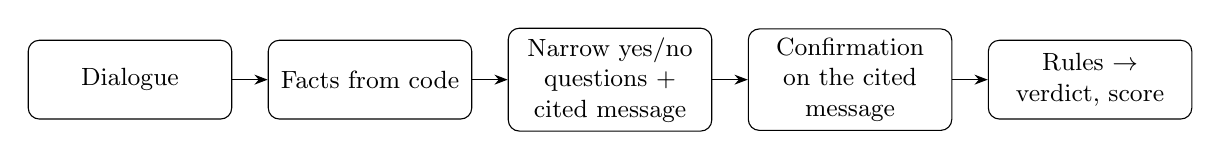
\begin{tikzpicture}[node distance=0.45cm, every node/.style={draw, rounded corners, align=center, font=\small, minimum height=1cm, text width=2.35cm}, >={Stealth}]
\node (d) {Dialogue};
\node[right=of d] (f) {Facts from code};
\node[right=of f] (q) {Narrow yes/no\\questions + cited message};
\node[right=of q] (c) {Confirmation\\on the cited message};
\node[right=of c] (r) {Rules $\rightarrow$\\verdict, score};
\draw[->] (d) -- (f); \draw[->] (f) -- (q); \draw[->] (q) -- (c); \draw[->] (c) -- (r);
\end{tikzpicture}
\caption{The evaluation pipeline. The LLM answers only the narrow questions.}
\end{figure}

\paragraph{Narrow questions.} Each criterion is split into yes/no questions; for example 07 (closing) asks
whether the chat was cut off by the client, whether the operator summarised the outcome, offered further
help and said goodbye. A question shows the model only the messages it needs (the first operator reply for
01, the whole dialogue for 04). The output is a JSON object constrained by a schema: \texttt{why} (reasoning,
written first), \texttt{answer} (boolean) and \texttt{message}, restricted to IDs that exist in the
dialogue---the model cannot cite a message that is not there.

\paragraph{Rules.} The checklist logic is code. For 07: N/A if the client left; otherwise yes iff
(summary or offer of help) and goodbye. Scale criteria are built from boolean facts level by level (06:
level 10 unless a lapse is found; a lapse is confirmed by a second question on the cited message, because the
model otherwise confuses rudeness, which belongs to 05 and 08, with incoherence). Unambiguous cases are
decided without the model. The score follows the checklist formula with N/A weights redistributed.

\paragraph{New criteria.} A reviewer may change the checklist. A criterion that does not match a built-in one
goes to a generic evaluator: applicability (N/A) in a separate call, then the answer from the rule's wording.
Deciding N/A in the same call made the small model pick ``na'' after reasoning that the criterion applied.

\paragraph{Baseline.} The standard LLM-as-a-judge: the whole dialogue, the checklist text and its general
rules in one prompt; for every criterion the model writes \texttt{why}, \texttt{answer} from the allowed values and
cited messages. It uses the same model, decoding settings, dialogue rendering and checklist text.

\paragraph{Settings.} \texttt{qwen3.5:9b}~\cite{qwen3} (Q4\_K\_M) on Ollama 0.40.5, temperature 0, seed 42,
context window sized to the prompt (8k--32k tokens), up to 384 output tokens per question (doubled when an
answer is cut off), RTX 4070 Laptop GPU (8\,GB). All prompts are in \texttt{ml/maestro/probes.py},
\texttt{generic.py} and \texttt{baseline.py}.

\section{Experimental protocol}
Metric: share of the 104 TEST labels where the system equals the human (exact match; for scales the level
must match). It is the quantity the reviewer cares about and treats N/A as a label of its own. We also report
the mean absolute error of the final score, precision and recall of the gross-violation flag, latency, LLM
calls and tokens per dialogue. Labels of one dialogue are correlated, so 95\% confidence intervals are
computed by bootstrap over dialogues~\cite{efron1993bootstrap} (2000 resamples); the comparison of the two
systems uses a paired bootstrap on the same dialogues. Both systems were run once at temperature 0 with the
same seed; run with \texttt{ml/eval/experiments.py}.

\section{Results}\label{sec:results}
\begin{table}[h]\centering\small
\begin{tabular}{lccccc}
\toprule
System & Agreement & 95\% CI & Score MAE & s/dialogue & LLM calls\\
\midrule
One-prompt judge (baseline) & 69.2\% & 59.6--77.9\% & 12.1 & 14.3 & 1\\
Proposed pipeline & \textbf{85.6\%} & 76.9--93.3\% & 11.0 & 34.7 & 17.4\\
\bottomrule
\end{tabular}
\caption{TEST, 13 dialogues, 104 labels, \texttt{qwen3.5:9b}, temperature 0. Paired difference (pipeline
$-$ baseline): $+16.3$ points, 95\% CI $[+5.8, +26.9]$; the difference was positive in
$\geq 99.5\%$ of 2000 bootstrap resamples. The
pipeline result equals an earlier independent run of the same code (85.6\%).}
\label{tab:main}
\end{table}

\begin{table}[h]\centering\small
\begin{tabular}{lcccccccc|ccc}
\toprule
 & 01 & 02 & 03 & 04 & 05 & 06 & 07 & 08 & RU & KZ & EN\\
\midrule
Baseline & 12 & 6 & 12 & \textbf{1} & 11 & 8 & 9 & 13 & 77\% & 66\% & 58\%\\
Pipeline & 13 & 7 & 11 & 11 & 12 & 10 & 13 & 12 & 81\% & 91\% & 88\%\\
\bottomrule
\end{tabular}
\caption{Correct labels per criterion (out of 13) and agreement per language (RU 6, KZ 4, EN 3 dialogues).}
\label{tab:crit}
\end{table}

\paragraph{Per criterion and language.} The baseline loses most on 04 (consultation): in 12 of 13 dialogues
it answered N/A (``no request was formulated'') although the client had asked a question, and on 07
(closing). In a single holistic answer the model applies N/A conditions loosely; the pipeline decides
applicability with a dedicated question and the rules. The baseline is also weaker on Kazakh and English
than on Russian, while the pipeline is not (with 3--6 dialogues per language these differences are
indicative only). The final-score error is similar for both (MAE 11.0 vs 12.1): an N/A answer removes a
criterion and re-weights the rest, so many label errors move the score less than the label agreement
suggests.

\paragraph{New criteria.} With four criteria replaced by ones the pipeline had never seen (TEST-NEW), the
generic evaluator agreed on 86.5\% of labels. A variant that decomposed each new criterion into
model-generated sub-conditions reached 76.9\% and was rejected.

\paragraph{Error analysis.} The pipeline disagrees with the annotator on 15 labels:
\begin{itemize}\itemsep0pt
\item \emph{Applicability of 02} (6 errors): whether the client gave enough information from the start
(N/A) or the operator had to ask. The checklist wording allows both readings; the pipeline never answered
``yes'' wrongly here: it predicted N/A three times and ``no'' three times where the annotator saw it otherwise.
\item \emph{Missed or false lapse in 06} (3): two missed lapses (level 7 labelled, 10 predicted) and one
false ``the client had to ask again'' (10 labelled, 4 predicted).
\item \emph{Identification and disclosure} (3): in t-ru-02 the operator disclosed account details without
identification; the pipeline judged identification not needed (N/A) but still flagged a confidential
disclosure in 08, an inconsistency between the two rules (the annotator marked 03 ``no'' and 08 ``no''). In
t-ru-06 the pipeline required identification where the annotator did not.
\item \emph{Partial credit in 04} (2): one too strict (20 labelled, 15 predicted), one too lenient (a wrong
answer got 10 instead of 0); \emph{empathy} (1): a missing reaction to a complaint was not noticed.
\end{itemize}
Most errors concern conditions that a second human could also read differently (02, the boundary between
03 and 08), which points to measuring inter-annotator agreement as the next step.

\paragraph{Negative results.} The model's thinking mode exceeded 4\,096 tokens per question and was not usable
within the latency budget. Giving the generic evaluator the checklist's general notes lowered its agreement
(71\%\,$\rightarrow$\,53\% on a development criterion), so it receives only rules added by the user.

\section{Optimisation and resources}
The deployed configuration runs Ollama with FlashAttention~\cite{dao2022flashattention} and an 8-bit KV
cache, which keep the 9B model and an 8k--16k context within 8\,GB of GPU memory. We did not measure the
configuration without them on the test set, so their effect on latency and quality is not quantified here.
Measured with the flags: 34.7\,s per dialogue (mean
over 13), 6.3\,GB of model memory of which 5.5\,GB on the GPU, 13\,032 prompt and 1\,044 output tokens in 17.4
calls per dialogue. The baseline needs 1\,779 prompt tokens and one call (14.3\,s): the pipeline trades
2.4$\times$ latency and 7$\times$ tokens for $+16$ points of agreement and stays within the 60\,s budget.
For comparison, the same pipeline on a cloud model (gpt-4.1-mini) took about 14\,s and \$0.006 per dialogue.

\section{Responsible use and limitations}\label{sec:responsible}
\paragraph{Risks.} (1) Wrong low scores can affect operators' bonuses; (2) the model may be weaker on Kazakh
than on Russian; (3) dialogues contain personal data; (4) a reviewer may over-trust an automatic score.
\paragraph{Mitigations.} Every verdict cites its evidence and the cited ID must exist; operators can appeal any
criterion and a reviewer decides with a reason while the model's answer stays visible; gross violations and low
scores go to a review queue rather than to automatic action; the default model is local, and personal data
(IIN, cards, phones, e-mails, IBAN) is masked before any cloud model.
\paragraph{Checks.} \emph{Masking} (\texttt{ml/eval/pii\_check.py}): on 24 hand-written cases in Russian,
Kazakh and English, 16 of 17 personal values were masked---the miss is an international phone number with a
four-digit group (\texttt{+44 20 7946 0958})---and none of 9 look-alike numbers (amounts, dates, order numbers,
an ISIN, a confirmation code) was masked. The missed format is a known gap; the fix is a broader phone
pattern, to be checked on the same cases. \emph{Language fairness}: the pipeline agrees with the annotator on
81\% of RU, 91\% of KZ and 88\% of EN labels (Table~\ref{tab:crit}); we see no disadvantage for Kazakh, but with
3--6 dialogues per language this is not conclusive. \emph{Over-trust}: the reviewer sees the cited message for
each verdict and the review queue ranks dialogues by gross violations and low scores.
\paragraph{Limitations.} The test set is small (13 dialogues; the interval is wide). Criterion 02 was changed
after the first TEST run. Financial facts in answers (tariffs, procedures) are not verified---there is no
knowledge base. Kazakh explanations were not reviewed by a native speaker. GPU inference is not bit-exact.

\section{Conclusions}
Splitting checklist criteria into narrow, evidence-bound questions and moving the verdict logic into code
lets a 9B open model on a laptop reach 85.6\% agreement with a human reviewer on unseen dialogues,
16 points above the one-prompt judge with the same model, at zero cost and with every verdict traceable to
a message. The accuracy, latency and cost targets of Section~1 are met, with the caveat that the test set
is small; the evidence target holds by construction of the output schema but was not audited separately. Next steps: a larger independently labelled test set with two annotators to
measure human agreement, and a knowledge base for factual checks in criterion 04.

\section*{Contributions and reused components}
\begin{tabularx}{\linewidth}{lX}
\toprule
Member / source & Contribution\\
\midrule
A. Zhumazhanov & ML pipeline (\texttt{ml/maestro}: questions, rules, generic evaluator, scoring, LLM clients),
baseline and experiment scripts (\texttt{ml/maestro/baseline.py}, \texttt{ml/eval/experiments.py}), Sections 4--7\\
T. Zholtayev & Data analysis and leakage check (\texttt{ml/eval/data\_analysis.py},
\texttt{ml/results/data\_analysis.md}), Section 3\\
A. Khamidulla & Personal-data masking check and responsible-use analysis (\texttt{ml/eval/pii\_check.py},
\texttt{ml/results/pii\_check.md}), Section 8\\
Reused & Web UI and backend (A.~Aspandiyar, B.~Serikov, A.~Islyamov); parts of \texttt{ml/} (A.~Aspandiyar);
TEST labels (A.~Islyamov)\\
Tools & Claude Code as a coding assistant, Gemini Pro for development labels; all code reviewed and tested
by the authors\\
\bottomrule
\end{tabularx}

\paragraph{Reproducibility.} Code, prompts, data and exact dependency versions (\texttt{ml/uv.lock}) are in the
repository; \texttt{uv run python eval/experiments.py run -{}-tag main} followed by \texttt{report} reproduces
Table~\ref{tab:main}.

\bibliographystyle{plainnat}
\bibliography{references}
\end{document}
